
\chapter{Anleitung zur Benutzung des Java-Interpolators}
\minitoc
\newpage
\section{Einleitung}
Im Rahmen meiner Diplomarbeit entstand, neben einer neuen Algebra f"ur SECONDO, auch eine Java-Anwendung, die die selbe Arbeitsweise wie die Algebra aufweist. Die Benutzung dieses Tools werde ich im Folgenden erl"autern.

Das Tool dient lediglich dem besseren Verst"andnis, wie die Algebra funktioniert. Ein Import oder Export mit SECONDO ist nicht m"oglich.
\section{Starten des Tools}
Das Tool ist in Java geschrieben, und wird als Jar-Datei verteilt. Um das Programm ausf"uhren zu k"onnen muss deshalb eine Java Laufzeitumgebung vorhanden sein. Ist dies der Fall, so l"asst sich das Programm mittels \begin{verbatim}
java -jar MCInterpolator.jar
\end{verbatim}  starten.

Es erscheint der Startbildschirm Abbildung \ref{fig:start}.

Dieser l"asst sich in vier Bereiche unterteilen:
\begin{itemize}
\item Eine Toolbar, die den Vrml-Export Button und den Zeit-Einsteller beinhaltet. 
\item Die Zeichen-Toolbar n"ahere Informationen zu dieser finden sich im Kapitel: ,,Zeichnen einer Region``
\item Der Zeichenbereich hier k"onnen Sie neue Regions zeichnen,und importierte Regions betrachten
\item Die Umschaltfl"achen, hier k"onne Sie zwischen den verschiedenen Werkzeugen wechseln. Nach dem Starten findet sich hier neben der Zeichenf"ache nur Konfigurationsschaltfl"ache, die im Kapitel: ,,Konfigurieren des Matchings`` n"aher beschrieben wird. Schlie"st man die Zeichnung von zwei Regions ab, so tauchen weitere Schaltfl"achen auf, die im Kapitel: ,,Die verschiedenen Ergebnisansichten`` erl"autert werden.
\end{itemize} 

\begin{figure}
   \centering
   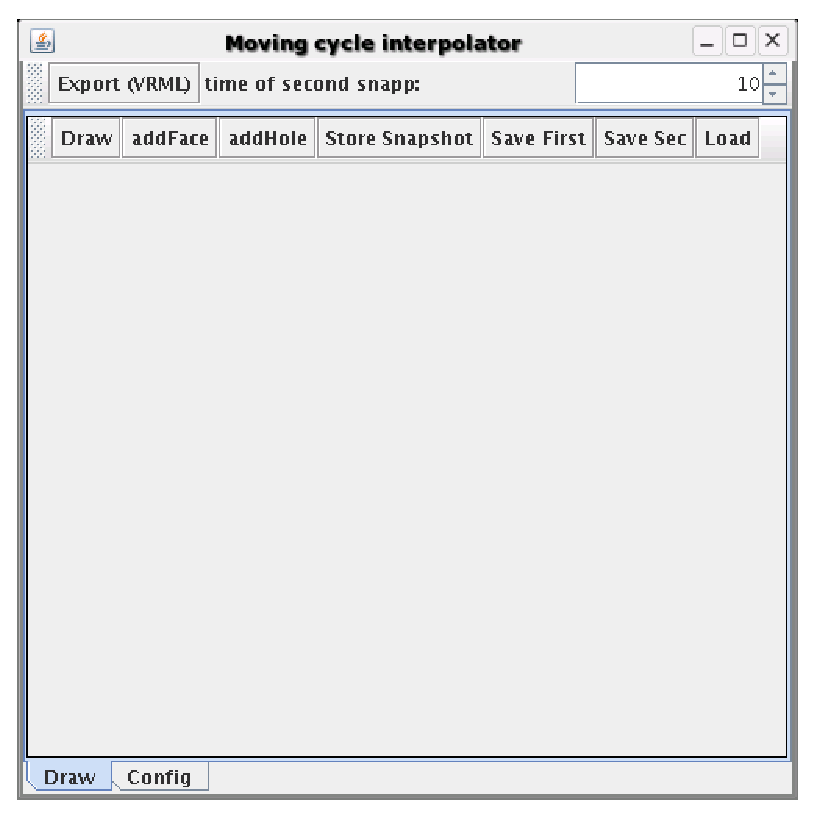
\includegraphics[scale=.8]{/home/java/Documents/Tex/Tex/start.eps}
   \caption{Der Startbildschirm}
   \label{fig:start}
\end{figure}

\section{Zeichnen einer Region}
\setcounter{section}{1}
Direkt nach dem Starten der Anwendung kann man anfangen, das erste Face zu zeichnen.  Das Zeichnen geht immer so vorsich, dass man die Punkte des Polygons nacheinander mit der Maus anklickt. Der neue Punkt, und die dazugeh"orige Linie werden direkt dargestellt. 

Das Polygon muss nicht geschlossen werden, aber bitte beachten Sie, dass alle Polygone einfache Polygone sein m"ussen. Eine entsprechende "Uberpr"ufung findet nicht statt.

Zum Zeichnen einer Region stehen folgende Werkzeuge bereit:
\begin{itemize}
\item Draw

Dieser Button l"oscht alle bereits eingegebenen Zeichnungen, und hinterl"asst ein leeres Zeichenblatt. Auch die eventuell bereits vorhandenen Schaltfl"achen f"ur die Ergebnissansichten werden ausgeblendet.
\item addHole

Hiermit kann man dem letzten Face ein Hole hinzuf"ugen. Holes unterscheiden sich von Faces darin, dass sie nicht blau sondern rot sind. Ein Hole muss komplett innerhalb seines Faces liegen, dies sicherzustellen ist die Aufgabe des Benutzers, eine "Uberpr"ufung findet nicht statt.
\item StoreSnapshot

Wollen Sie die Zeichnung einer Region beenden, so klicken Sie bitte auf diesen Button. Falls es der erste Schnappschuss ist, den Sie beenden, so f"arbt sich dieser blasser, und sie k"onnen den n"achsten zeichnen. Beenden Sie aber den Zweiten, so wird das passende Match berechnet, und in den zus"atzlichen Schaltfl"achen dargestellt, die Sie in ,,Die verschiedenen Ergebnisansichten`` finden.
\end{itemize} 
\section{Importieren- Exportieren}
Zum Importieren und Exportieren von Schnappsch"ussen, die Sie mit diesem Programm erzeugt haben stehen drei Schaltfl"achen zur Verf"ugung:

,,Save First``, ,,Save Sec`` und ,,Load``. Klicken Sie auf einen der beiden Save-Buttons, so "offnet sich ein Dateiauswahl-Dialog, in dem Sie einen Dateinamen f"ur die Schnappschuss-Datei angeben k"onnen.

Mit Hilfe des Load-Buttons k"onnen Sie dann diese SSchnappsch"usseeinzeln wieder laden. Falls Sie bereits zwei Schnappsch"usse in dem PProgrammhaben, so dr"ucken die bitte ,,Draw``, bevor Sie neue Dateien einlesen.
\section{Konfigurieren des Matchings}
Hinter der SSchaltfl"ache ,,Config`` verbirgt sich ein Dialogfenster (siehe Abbildung \ref{fig:Config}), in dem einige Einstellungen vorgenommen werden k"onnen:
\begin{itemize}
\item VRML Filename und VRML Application

Erl"auterungen zu diesen Feldern finden Sie in dem Unterkapitel: ,,Die verschiedenen Ergebnisansichten / Vrml-Export``
\item Auswahlfeld f"ur die Art des Matchings

Hier kann man ausw"ahlen, welches Matching man gerne ausf"uhren m"ochte. Die zur Zeit verf"ugbaren Matching-Methoden werden in der Arbeit ausf"uhrlich erl"autert.
\item Schieber f"ur die Parameter der Einzelmatches

Hier kann man einigen Einzel-Matches, zur Zeit dem OverlappingMatch und den Referenzpunktverfahren, einen Parameter "ubergeben. Bitte beachten Sie, dass dieser Parameter je nach der Art des Matches unterschiedliche Auswirkungen hat.
\item Schieber f"ur die Parameter des Optimalmatches

Das OtimalMatch setzt sich aus den EinzelMatches zusammen, indem es verschiedene Einzelmatches, mit verschiedenen Parametern, ausf"uhrt, und diese dann bewertet. In diese Bewertung flie"sen mehrere Kriterien gewichtet ein. Mit Hilfe dieser Schieber lassen sich die Gewichte der Einzel-Kriterien ver"andern.
\item Die Einzel-Bewertungen des Matches

In diesen Feldern finden Sie die Bewertungen des aktuellen Matches aufgeschl"usselt nach den einzelnen Kriterien.
\end{itemize} 
\begin{figure}
   \centering
   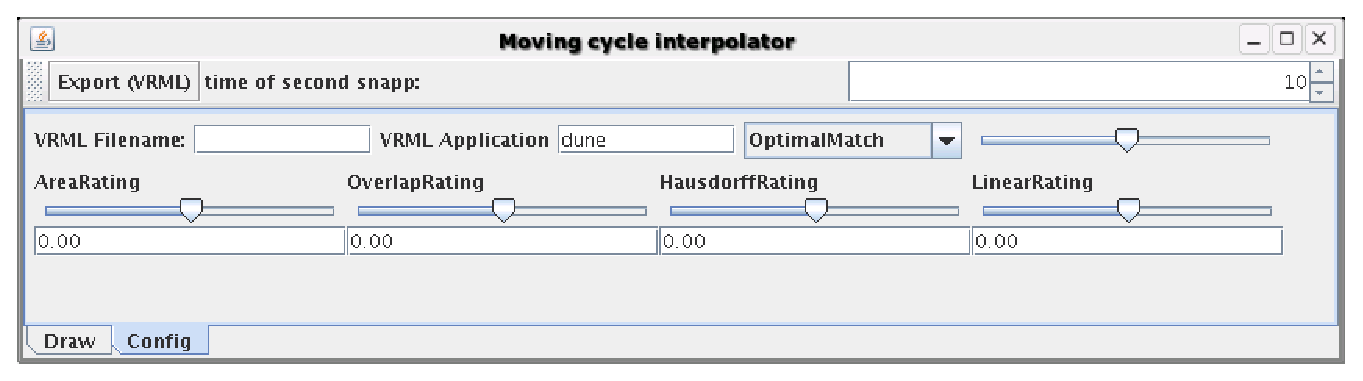
\includegraphics[scale=.65]{/home/java/Documents/Tex/Tex/Config.eps}
   \caption{Der Config-Dialog}
   \label{fig:Config}
\end{figure}
\section{Die verschiedenen Ergebnisansichten}
SoSobalder zweite ScSchnappschussbgeschlossen wird, erscheinen einige neue Schaltfl"achen, in denen Sie das Resultat des Matchings finden.

Bei den Erl"auterungen dieser Schaltfl"achen benutze ich die ScSchnappsch"ussesie in Abbildung \ref{fig:Splits} dadargestelltind.
\begin{figure}
   \centering
   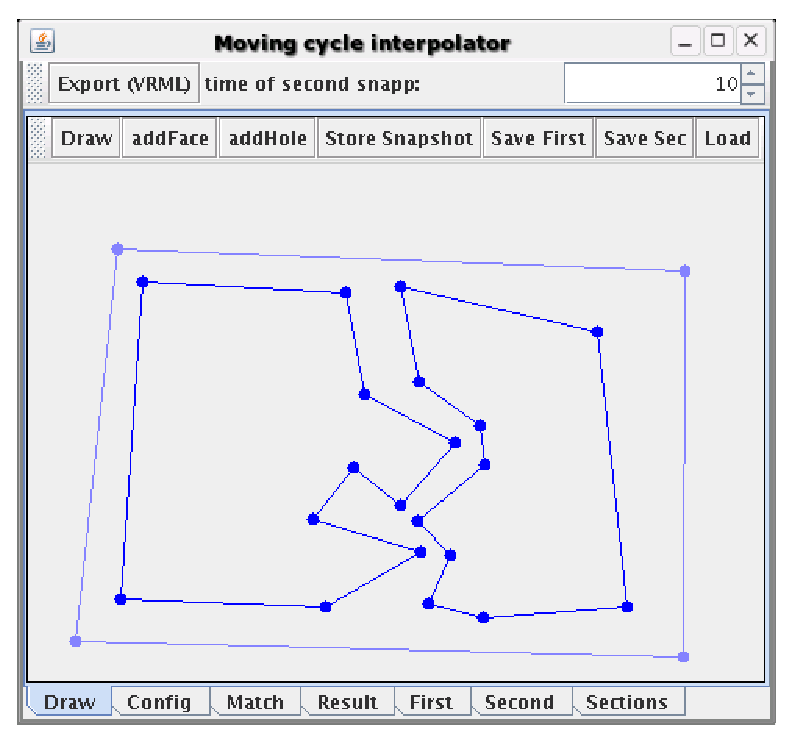
\includegraphics[scale=.8]{/home/java/Documents/Tex/Tex/Splits.eps}
   \caption{Das Beispiel}
   \label{fig:Splits}
\end{figure}
\subsection{Match}
In diesem Bildschirm (siehe Abbildung \ref{fig:Match}) finden Sie die beiden Schnappsch"usse in derselben Darstellung, wie in ,,First`` und ,,Second``. In dem entsprechenden Kapitel wird diese Darstellung n"aher erl"autert. 

W"ahlen Sie ein Element in einer der beiden Darstellungen aus, so wird das gematchte Element der anderen Darstellung selektiert. 

In der Rechten oberen Ecke des Fensters finden Sie den Namen des Matches, eine Erl"auterung zu diesem und die Bewertung in den Kategorien. Falls Sie ein OptimaMatch verwenden, so findet sich hier eine Liste mit allen Einzelmatches, die zu diesem ErErgebnisommen.
\begin{figure}
   \centering
   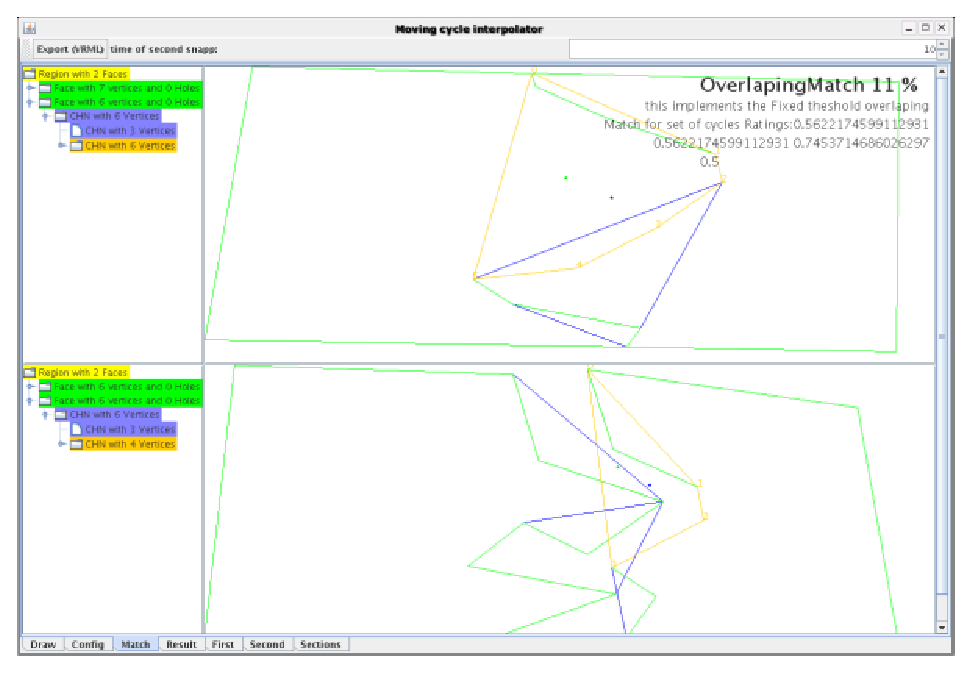
\includegraphics[scale=.8]{/home/java/Documents/Tex/Tex/Match.eps}
   \caption{Die Match-Darstellung}
   \label{fig:Match}
\end{figure}

\subsection{Result}
In diesem Bildschirm (siehe Abbildung \ref{fig:Result}) finden Sie eine isometrische Darstellung des Matches. Sie hier k"onnen Ihre bebeidenchnappsch"usse wiederfinden. Der Erste ist in blau gezeichnet, der Zweite in Rot. Die Linien, die die Beiden verbinden sind Grau. 

Mit Hilfe des Zeit-Einstellers in der obersten Toolbar k"onnen Sie den zweiten Schnappschusreiter nach hinten rechts verschieben, bzw. zur"uckholen. 

\begin{figure}
   \centering
   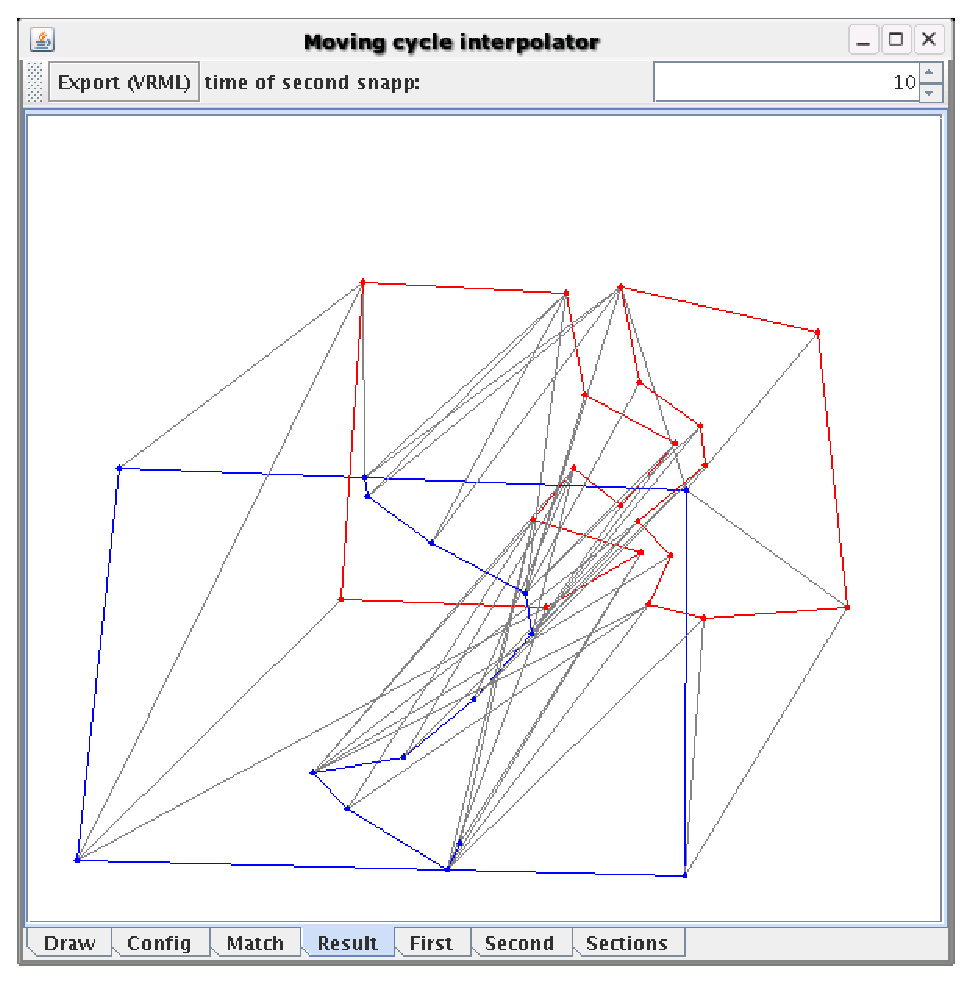
\includegraphics[scale=.6]{/home/java/Documents/Tex/Tex/Result.eps}
   \caption{Die Result-Darstellung}
   \label{fig:Result}
\end{figure}
\subsection{First und Second}
In dieser Ansicht (in Abbildung \ref{fig:Second} finden Sie ,,Second`` als Beispiel) finden Sie zwei Darstellungen des ConvexHullTrees eines Schnappschusses. Links finden Sie eine Baumansicht des ConvexHullTrees.

Diese Darstellung erm"oglicht es Ihnen, in dem Baum zu navigieren und Elemente zu selektieren. Mehrfachselektionen kann man vornehmen, indem man beim Klicken die Strg oder die UmUmschaltaste h"alt. Die einzelnen Elemente des Baumes sind farblich zu unterscheiden.

Die Farben bedeuten:
\begin{itemize}
\item Gelb Region
\item Gr"un Face
\item Blau ConvexHullTreeNode
\item Rot Hole
\item Orange Selektion
\end{itemize} 

Rechts finden Sie eine Darstellung des Baumes als Menge von Polygonen. Die Farbgebung entspricht der oben genannten, nur das die Region nicht extra dargestellt ist. Jedes Face ist durch das Polygon seines Cycles dargestellt, jedes Element eines ConvexHullTrees, einschlie"slich der Holes, ist durch seine konvexe H"ulle dargestellt. Selektiert man ein Element in der Baumansicht, so f"arbt sich dieses Orange, die Ecken der Konvexen H"ulle werden durchnummeriert und Schwerpunkt (blau) und Steiner-Punkt (gr"un) werden dargestellt.

\begin{figure}
   \centering
   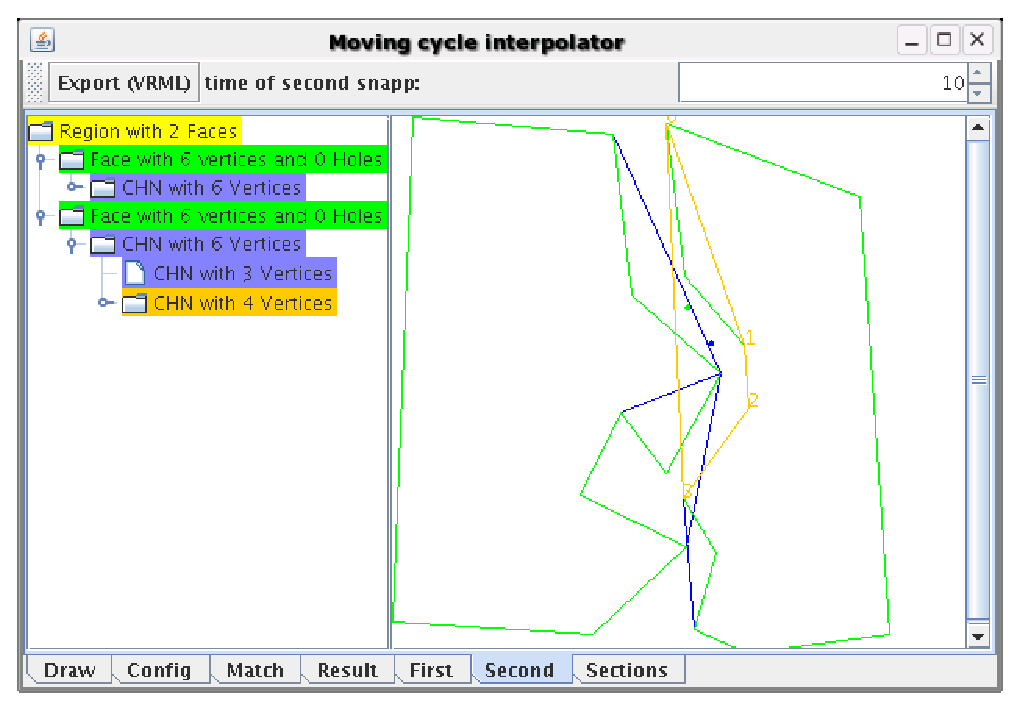
\includegraphics[scale=.8]{/home/java/Documents/Tex/Tex/Second.eps}
   \caption{Die ConvexHullTree-Darstellung des Zweiten Schnappschusses}
   \label{fig:Second}
\end{figure}
\subsection{Sections}
In dieser Darstellung (Abbildung \ref{fig:Sections}) finden Sie interpolierte Schnappsch"usse, die aus Ihrem Match erstellt wurden. In dem Feld mittig "uber der Darstellung k"onnen Sie w"ahlen, wieviele ScSchnappsch"usseie betrachten wollen. 

Diese tauchen dann in dem Zeichenbereich dieser Seite auf. Der Erste und der Letzte entsprechen dem ersten und dem zweiten Schnappschuss, den Sie eingegeben haben.
\begin{figure}
   \centering
   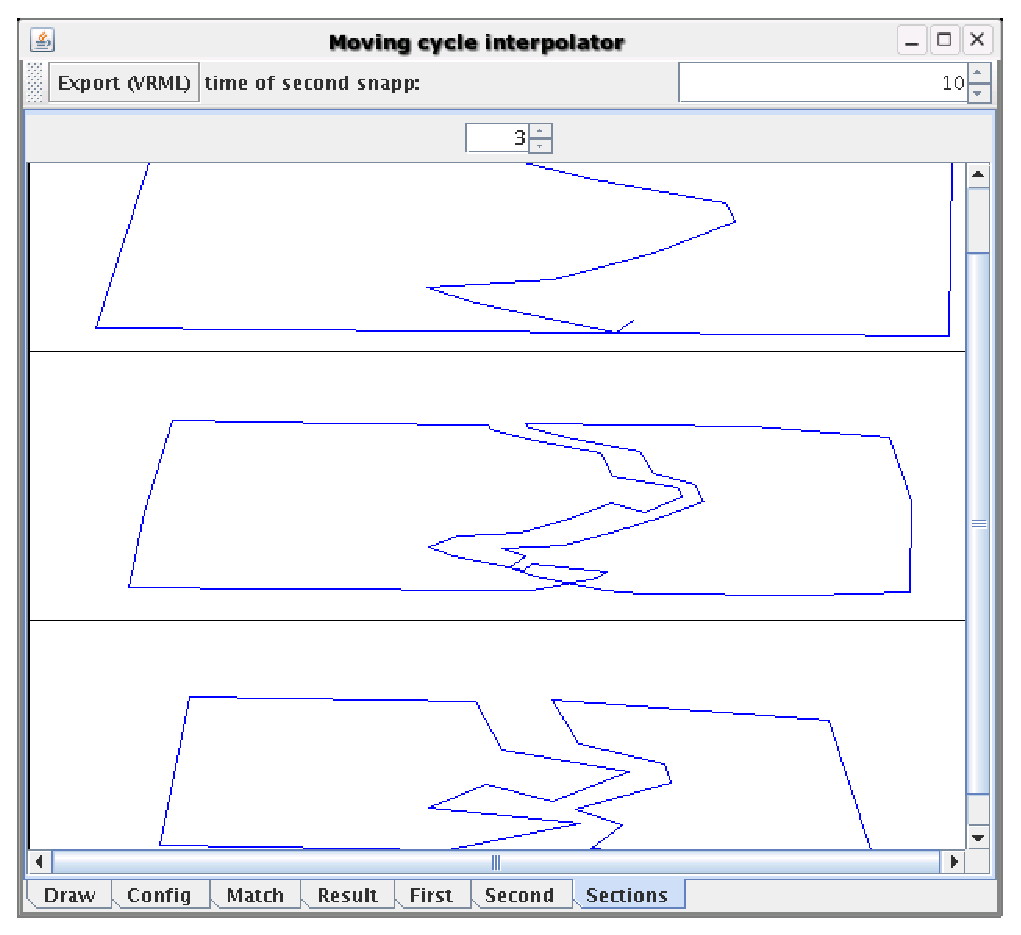
\includegraphics[scale=.8]{/home/java/Documents/Tex/Tex/Sections.eps}
   \caption{Drei Sections unseres Beispieles}
   \label{fig:Sections}
\end{figure}
\subsection{Vrml-Export}
Das Tool bietet die M"oglichkeit, ein Match in eine Vrml-Datei zu exportieren und so eine ansprechende 3D-Darstellung zu erhalten. Zu dem Vrml-Export geh"oren vier GUI-Elemente:
\begin{itemize}
\item VRML Filename im Config-Dialog

 In diesem Feld kann man den erw"unschten Dateinamen angeben, den die neue Vrml-Datei bekommen soll. Die Erweiterung .vrml wird automatisch ererg"anzt
\item VRML Application im Config-Dialog

Tr"agt man in diesem Feld einen Konsolenbefehl ein, mit dem man einen VRML-Viewer startet, so startet das Tool diesen Viewer direkt nach dem Export mit der neuen Datei.

\item Der ,,Zeit-Einsteller`` in der obersten Toolbar

Mit diesem Control k"onnen Sie die ,,H"ohe`` der 3D-Darstellung bestimmen. Kleine Werte f"uhren zu flachen Poyedern und Gro"se zu Hohen.
\item Der ,,Export (VRML)``-Button in der obersten Toolbar

Durch den Klick auf diesen Button wird der Export ausgel"ost. Die Vrml-Datei der gew"unschten H"ohe und mit dem gew"ahlten Namen wird erzeugt und direkt in dem Viewer Ihrer Wahl ge"offnet.
\begin{figure}
   \centering
   
\includegraphics[scale=1]{/home/java/Documents/Tex/Tex/vrml.eps}
   \caption{Das Beispiel in einem Vrml-Viewer}
   \label{fig:vrml}
\end{figure}
\end{itemize}
